\chapter{Additional Plots}
\label{appendix_supplemental}

In this section we show some useful plots in appendix of the study of magnetization profile, two-point correlation function and spin transport in the model analyzed.

\section{Supplemental Plots on Magnetization Profile}

As anticipated in section~\ref{sec:magn_profile}, along x and y direction the magnetization profile is trivial, because the dissipators act only along z direction. This is displayed in fig.~\ref{fig:comparisonSigmaXYZ} for a 8-sites chain with $J_z = 1$ and $\gamma = 1$, but it has been found the same result also for other parametrizations of the system.

\begin{figure}[H]
    \centering
    \captionsetup{width=1.\linewidth}
    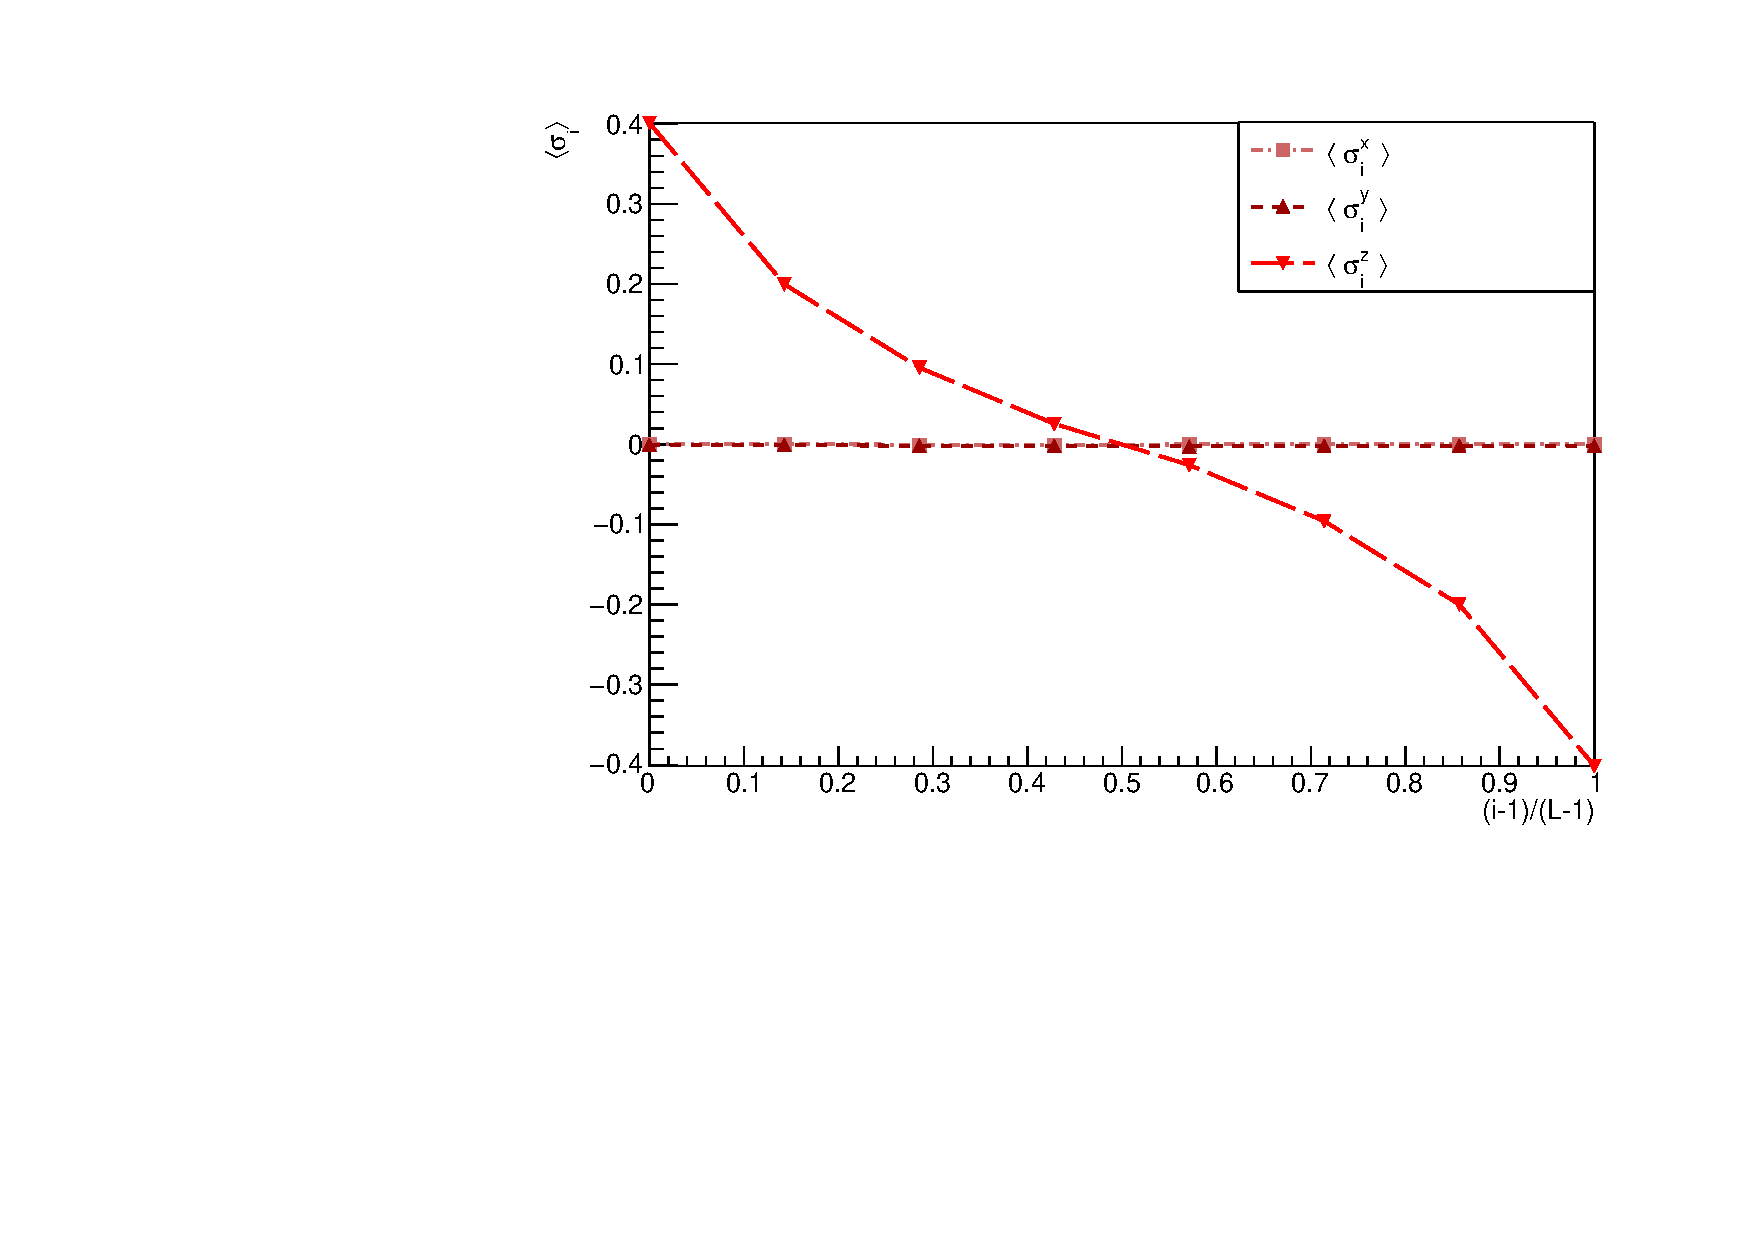
\includegraphics[scale=0.6]{Figures/comparisonSigmaXYZ.pdf}
    \caption{Magnetization profile along the x, y and z spin direction, for a 8-sites chain with $J_z = 1$ and $\gamma = 1$.}
    \label{fig:comparisonSigmaXYZ}
\end{figure}

The magnetization along z direction of every spin of the chain, increases with $\gamma$ following an exponential trend. This is confirmed also by the study of the gradient $\nabla \sigma^z$, the fit of which shows a dependence as the following:
\begin{equation*}
    \nabla \sigma^z (\gamma) = - p_0 + p_1 e^{-p_2\gamma},
\end{equation*}
as displayed in fig.~\ref{fig:FIT_12sites_gradLM34VSgamma}, for a 12-sites chain, for which the gradient between the third and the forth spins has been analyzed.
\begin{figure}[H]
    \centering
    \captionsetup{width=1.\linewidth}
    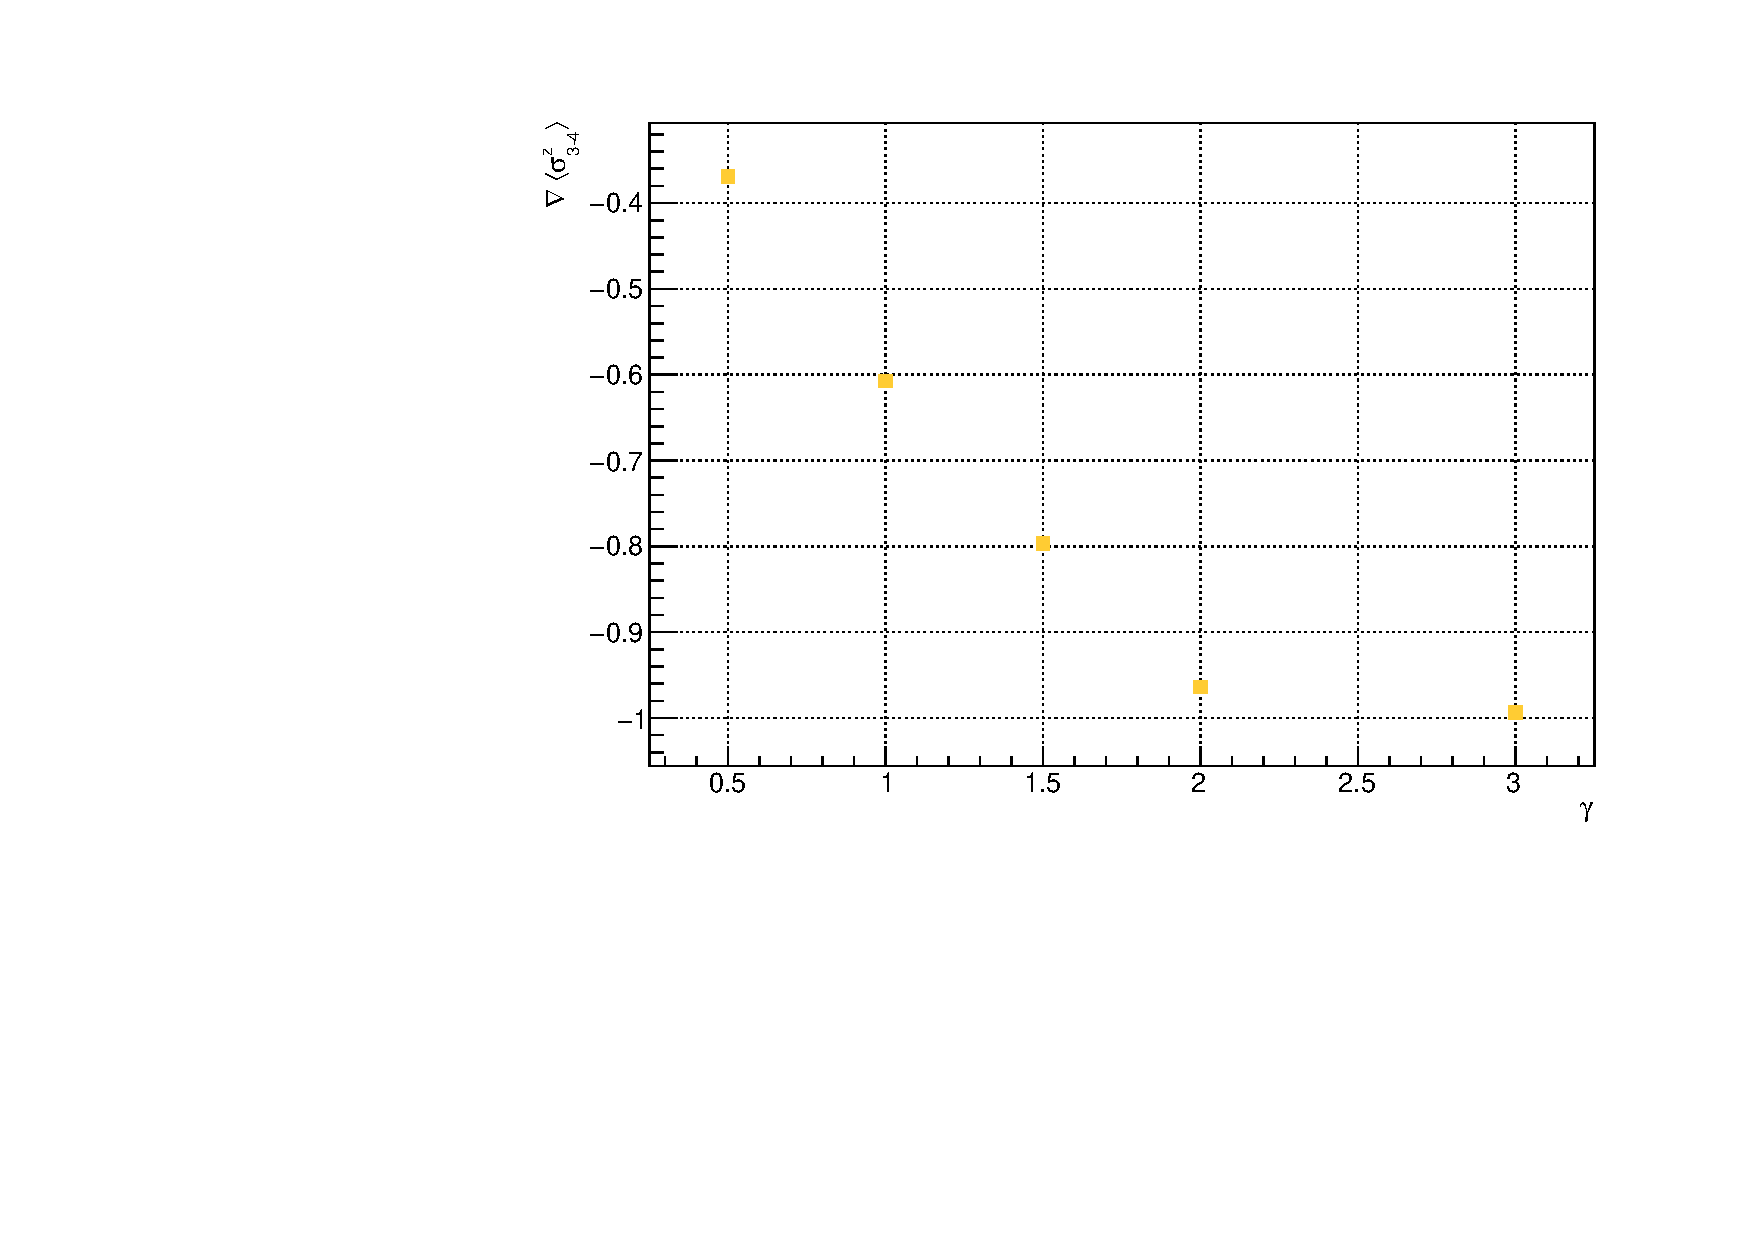
\includegraphics[scale=0.6]{Figures/12sites/12sites_gradLM_3and4VSgamma.pdf}
    \caption{Profile of the gradient between the third and the forth site of a 12-sites chain versus $\gamma$. The fit shows an exponential profile.}
    \label{fig:FIT_12sites_gradLM34VSgamma}
\end{figure}

Another feature mentioned in section~\ref{sec:magn_profile}, is the fact that while $\gamma$ grows, the expectation value of $\sigma^z$ tends asymptotically to a limit value, that depends on the site under consideration. In section~\ref{sec:magn_profile}, the coefficient that controls this rate has been named $p_1$. In fig.~\ref{fig:16sites_p1VSsiteIndex} we see that $p_1$ has a linear dependence on the site position.

%il primo punto è un effetto dovuto al bordo, dove risente della presenza del bagno c'è il dissipatore; il resto è costante. Da 5 in poi i punti sono molto vicini a zero, non li plttaimo perché abbiamo valori piccoli e non riusciamo ad avere uns tima accurata di p. Nel primo sito c'è un offset prob dovuto alla pres del bagno, perchè il sistem anon è omogeneo. Negli altri siti è praticamente costante. 

\begin{figure}[H]
    \centering
    \captionsetup{width=1.\linewidth}
    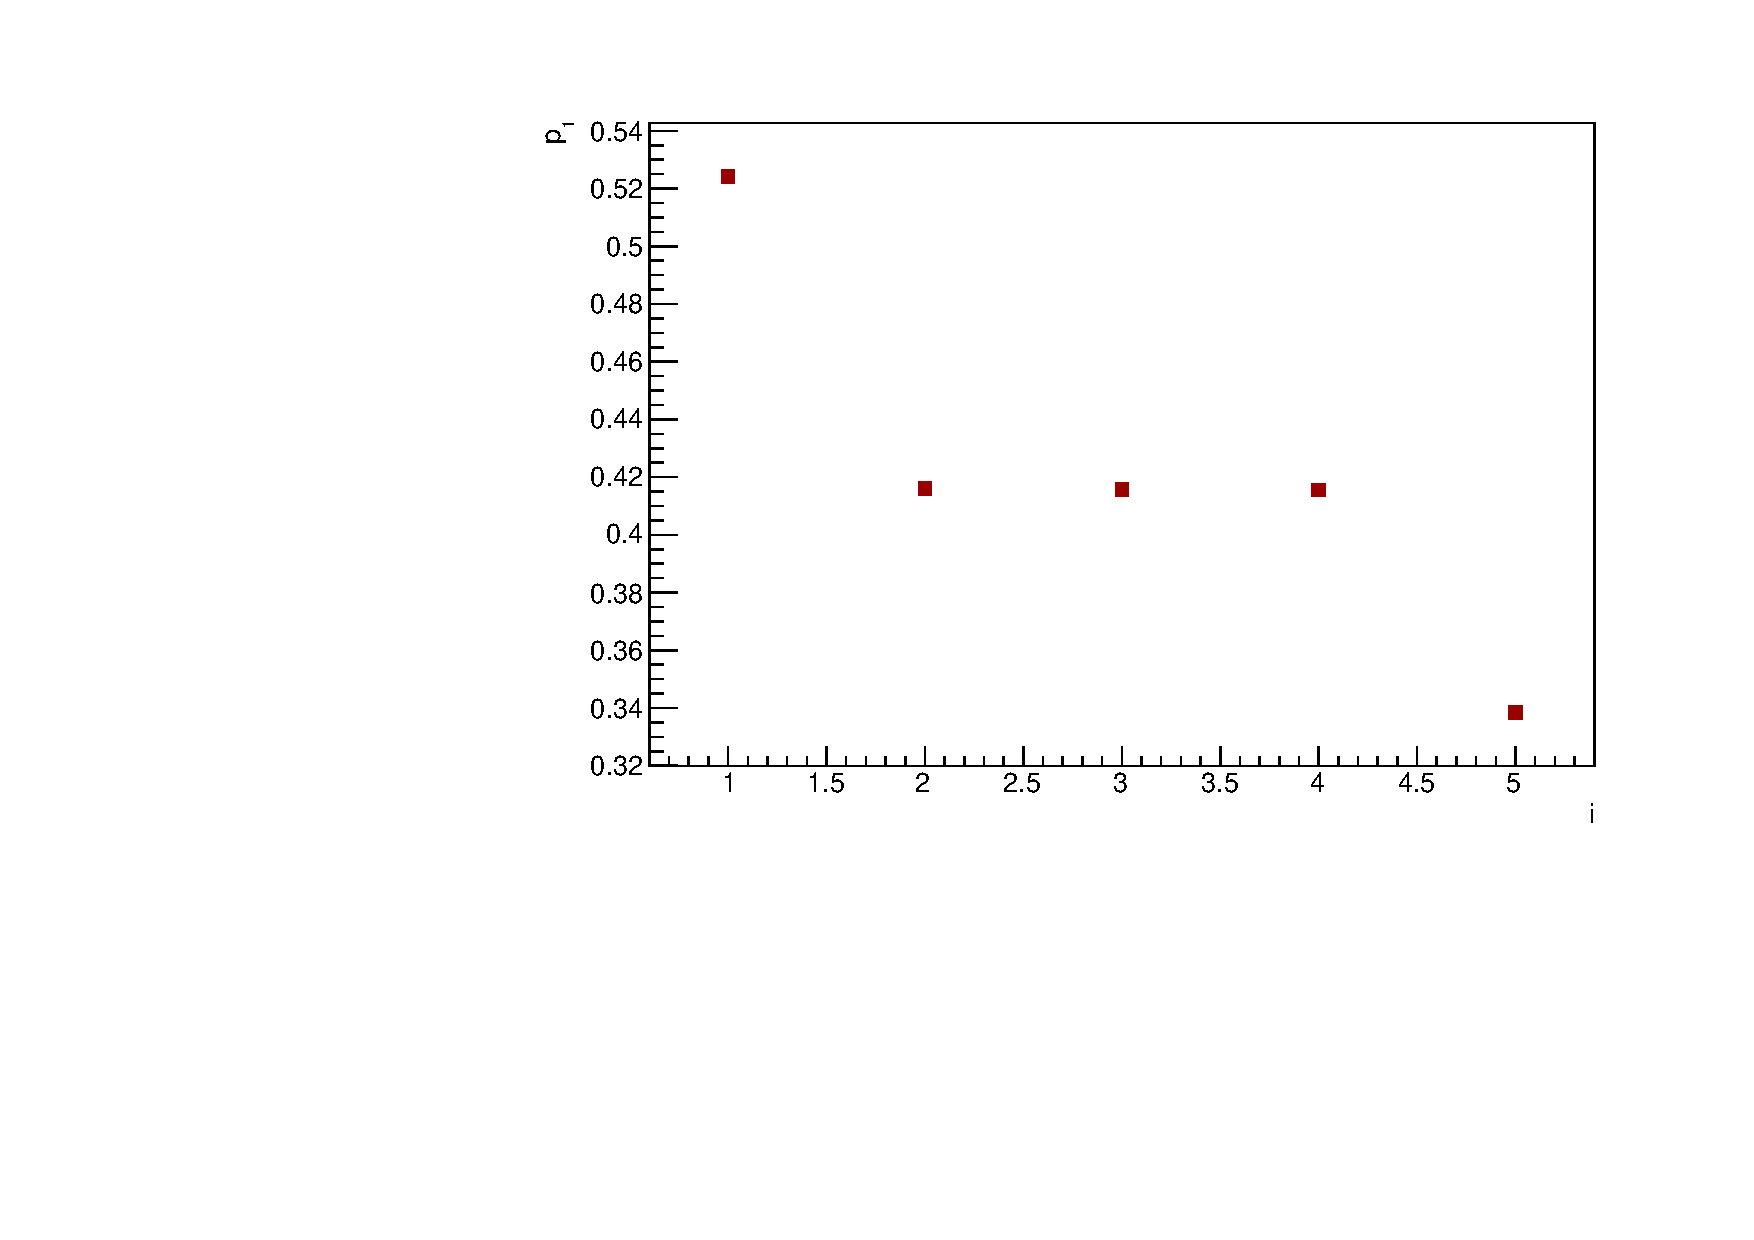
\includegraphics[scale=0.6]{Figures/16sites_p1VSsiteIndex.pdf}
    \caption{Growth rate coefficient $p_1$ versus site index. Beyond the fifth site the profile is no longer exponential because of the zero magnetization plateau.}
    \label{fig:16sites_p1VSsiteIndex}
\end{figure}

\section{Supplemental Plots on Correlations}
We have seen that the bulk correlation function, defined in section~\ref{sec:2P_correlationFunction}, has an exponential profile, with a decay rate coefficient $p_1$ that depends on $\gamma$, with a dependence shown in fig~\ref{fig:CFBulkCONN_p1vsGamma}. The non-monotonic profile is probably due to the competion between Hamiltonian dynamics and dissipative dynamics.

\begin{figure}[H]
    \centering
    \captionsetup{width=1.\linewidth}
    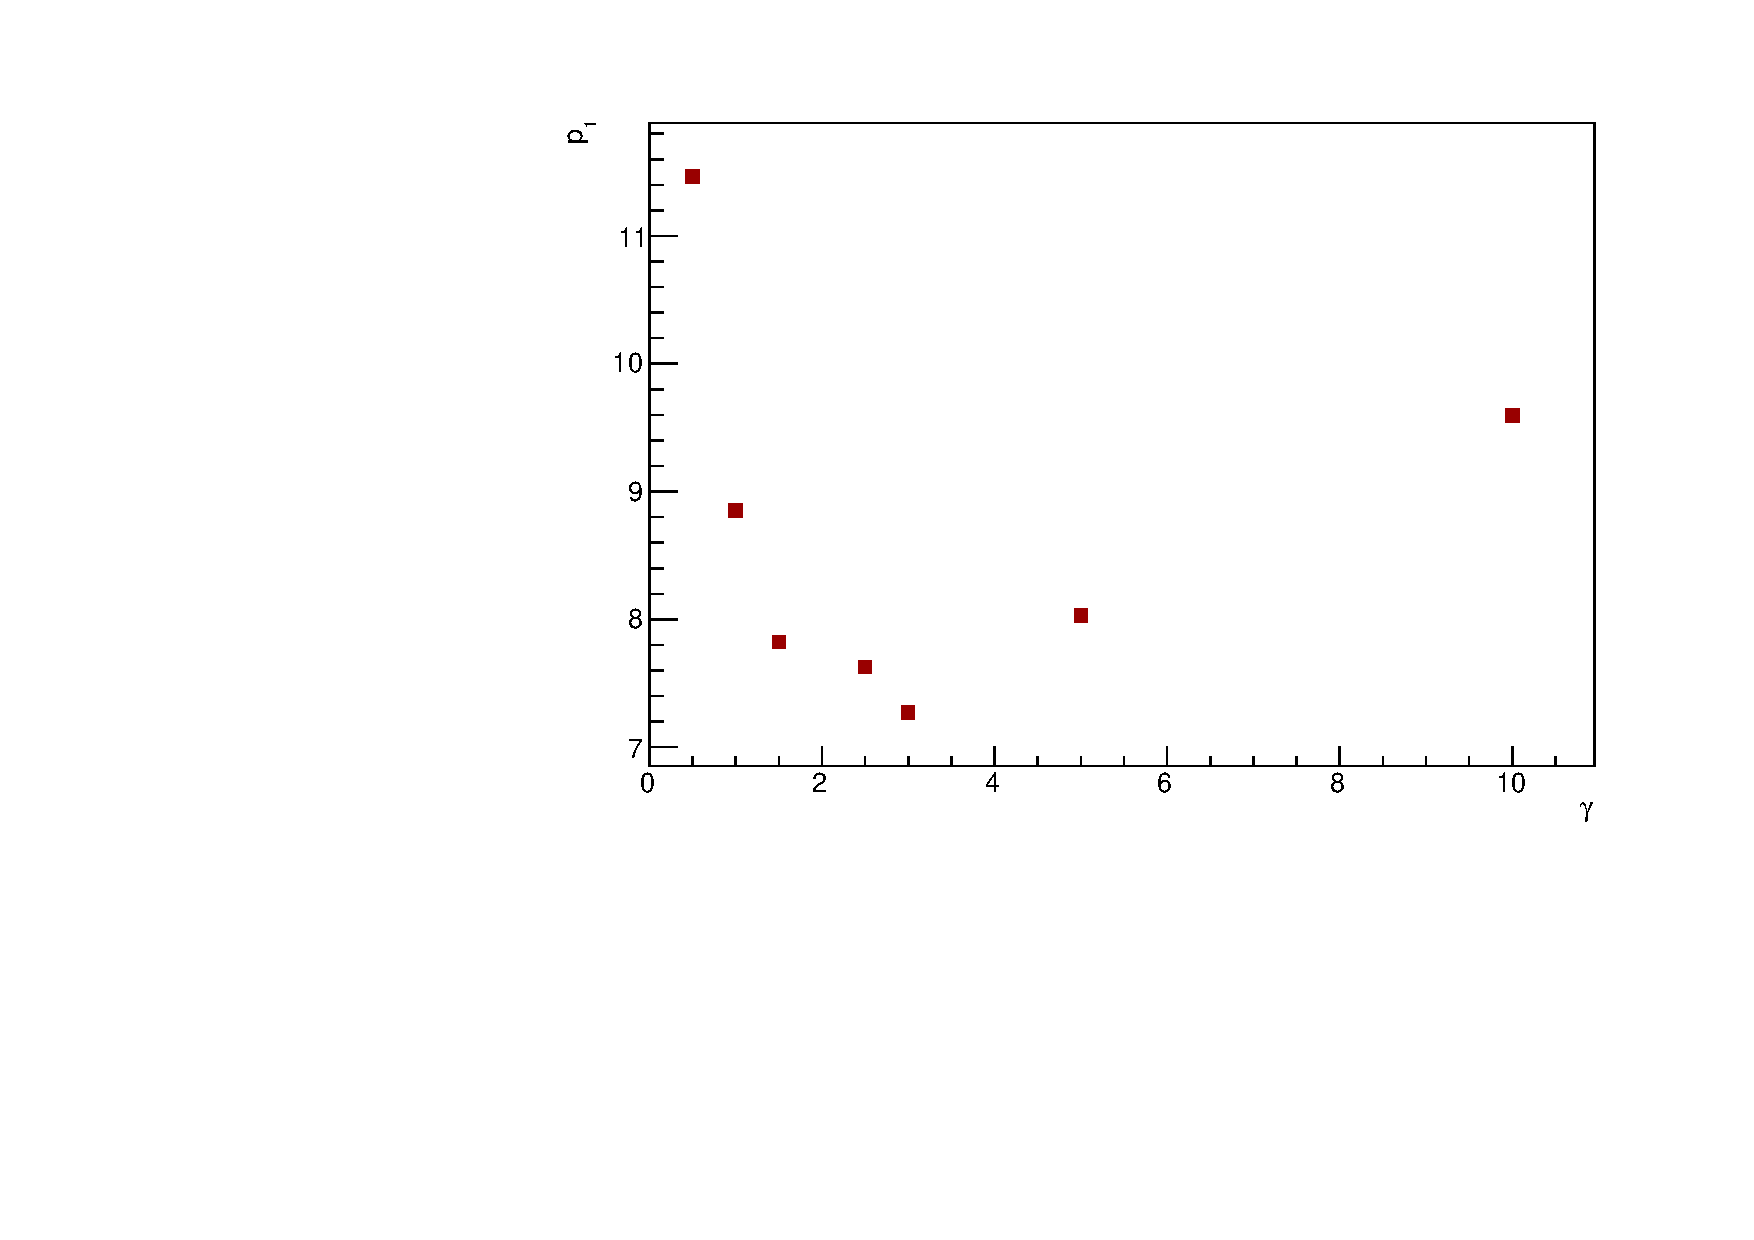
\includegraphics[scale=0.6]{Figures/CFBulkCONN_p1vsGamma.pdf}
    \caption{Rate coefficient $p_1$ versus $\gamma$. The trend is non-monotonic, due to the competition between the Hamiltonian and dissipative dynamics.}
    \label{fig:CFBulkCONN_p1vsGamma}
\end{figure}

\section{Supplemental Plots on Spin Transport}
As we have seen in section~\ref{spin_curr}, the spin current depends on $J_z$. The spin current between the first two spins and the last two spins of the chain is shown in fig.~\ref{fig:SpinCurrVSJz1st} and in fig.~\ref{fig:SpinCurrVSJzLth} respectively. 

It is clear that the peak values of spin current are independent of $J_z$ while $J_z < 0.9$; from $J_z \geq 1$, it rapidly decays to zero. This is probably due to the fact that if the Hamiltonian dynamics gets a predominant role over the dissipative dynamics,the system does not detect any driven effect, so it reacts like there was no dissipative forces.

\begin{figure}[H]
    \centering
    \captionsetup{width=1.\linewidth}
    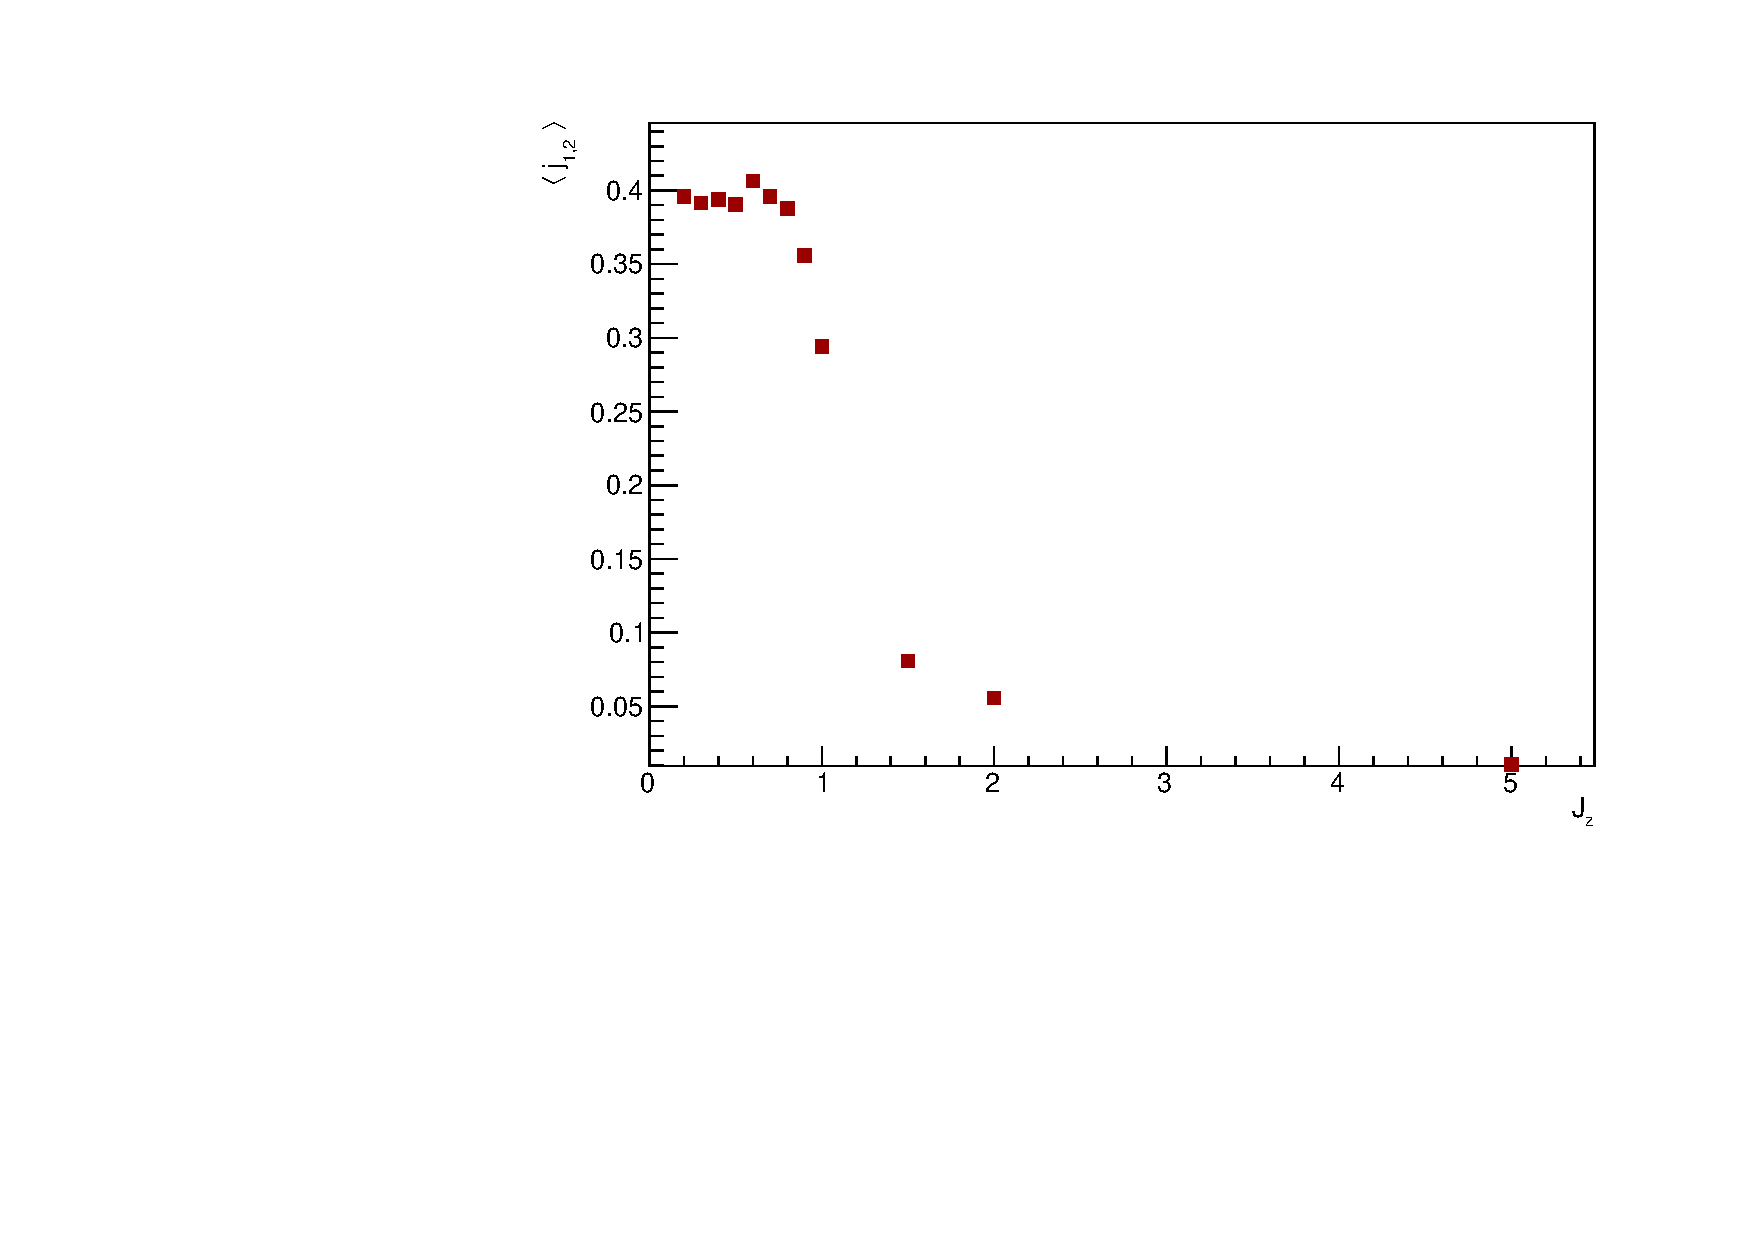
\includegraphics[scale=0.6]{Figures/SpinCurrVSJz1st.pdf}
    \caption{Spin current between the first two spins of a 16-sites chain, with $\gamma=1$ versus several values of $J_z$. Errors have been estimated as explained in section~\ref{sec:MPO_errors}.}
    \label{fig:SpinCurrVSJz1st}
\end{figure}

\begin{figure}[H]
    \centering
    \captionsetup{width=1.\linewidth}
    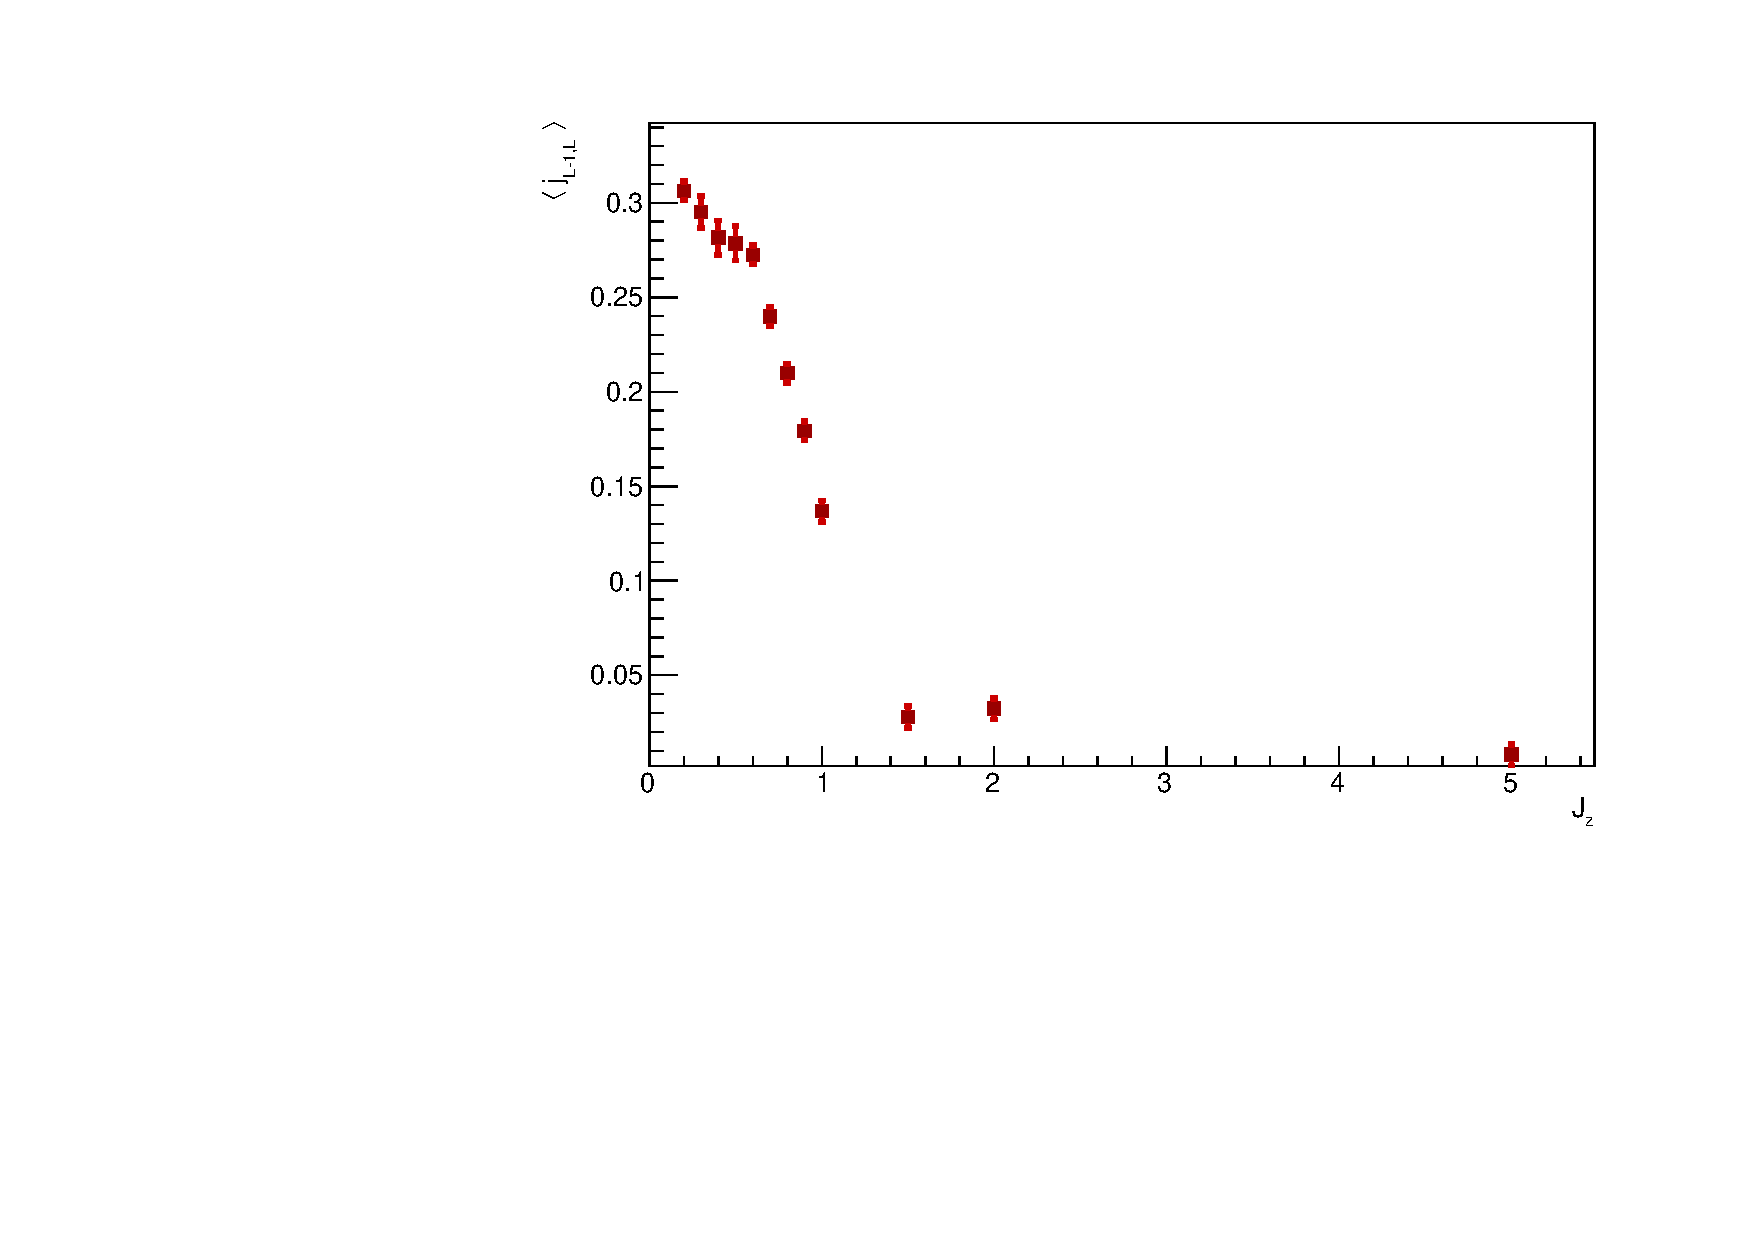
\includegraphics[scale=0.6]{Figures/SpinCurrVSJzLth.pdf}
    \caption{Spin current between the last two spins of a 16-sites chain, with $\gamma=1$ versus several values of $J_z$. In contrast to $j_{1,2}$, in this case there is a decreasing profile even for $J_z < 0.9$. This could be true or it be due to the difficulty on reaching convergence for this values of $J_z$. The numerical errors are displayed by the red error bars in the plot and they have been estimated as explained in section~\ref{sec:MPO_errors}.}
    \label{fig:SpinCurrVSJzLth}
\end{figure}